\documentclass[12pt, a4paper]{article}
\usepackage{fontspec}
\setmainfont{Times New Roman}
\usepackage[UTF8]{ctex}
\usepackage{listings}
\usepackage{array}
\usepackage{geometry}
\geometry{a4paper, scale=0.75}
\usepackage{ctex}
\usepackage{amsmath}
\usepackage{epsfig}
\usepackage{graphicx}
\usepackage{epstopdf}
\usepackage{cite}
\usepackage{indentfirst}
\setlength{\parindent}{2em}
\setlength\parskip{.3 \baselineskip}
\usepackage{graphicx}
\usepackage{float}
\usepackage{subfigure}

\begin{document}
	\begin{center}
		\vspace{0.2in}
		\noindent{\fontsize{20pt}{1em}\selectfont\textbf{通信电路\quad 第三周作业}} \\ [12pt]
		\noindent{\fontsize{20pt}{1em}\textbf{Cadence报告}}  \\ [12pt]
		{\fontsize{14pt}{1.2em}\selectfont
			刘开济\\ [10pt]
			2019010973 \\ [10pt]
		}
	\end{center}
    \section{用有源电路实现Butterworth Low Pass Filter}
    首先考察原形滤波器如下图:
        \begin{figure}[H]
    	\centering
    	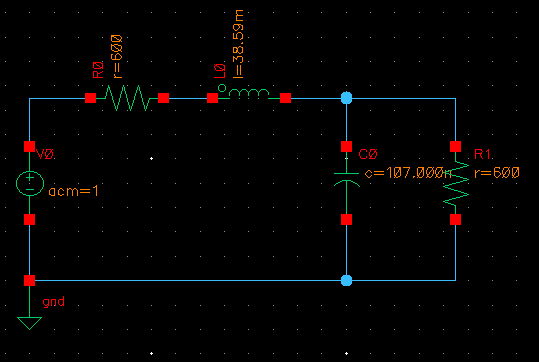
\includegraphics[width = 0.8\textwidth]{OriginalLPF}
    	\caption{原形低通滤波器}
    	\label{Fig2.1}
    \end{figure}\par
    记$R_S$上电压为$V_1$,输出电压为$V_2$,并记源电压为$V_s$,则不难得到积分电路方程:
    \begin{gather}
    	V_1  = \frac{1}{s (\frac{L}{R^2}R)}(V_s - V_1 - V_2)\\
    	V_2 = \frac{1}{sCR}(V_1 - V_2)
    \end{gather}\par
    由积分电路方程不难设计如下电路:
     \begin{figure}[H]
    	\centering
    	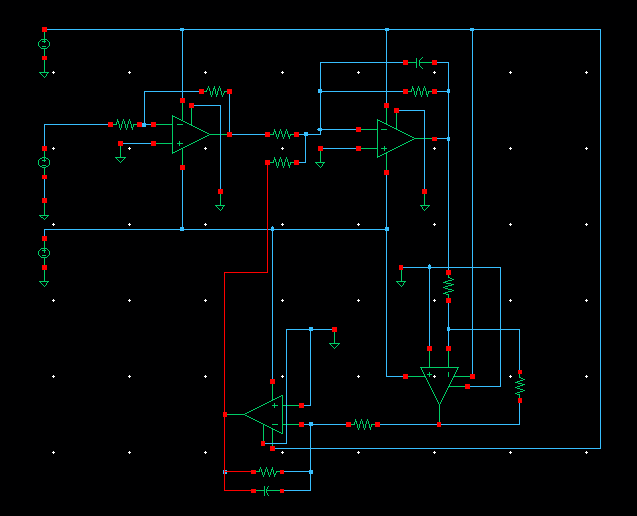
\includegraphics[width = 0.8\textwidth]{ActiveLPF}
    	\caption{有源低通滤波器}
    \end{figure}\par
    初始设置取OPA电压增益$A_v = 1000000$,输入电阻$r_{in} = 1M \Omega$,输入电阻$r_{out} = 1 \Omega$,单位增益频点$f_{unity \ gain} = 1MHz$。这里我们要说明,对于单极点运放,有$f_{unity \ gain} = \frac{1}{R_n C_n}$。有仿真图像如下:
     \begin{figure}[H]
    	\centering
    	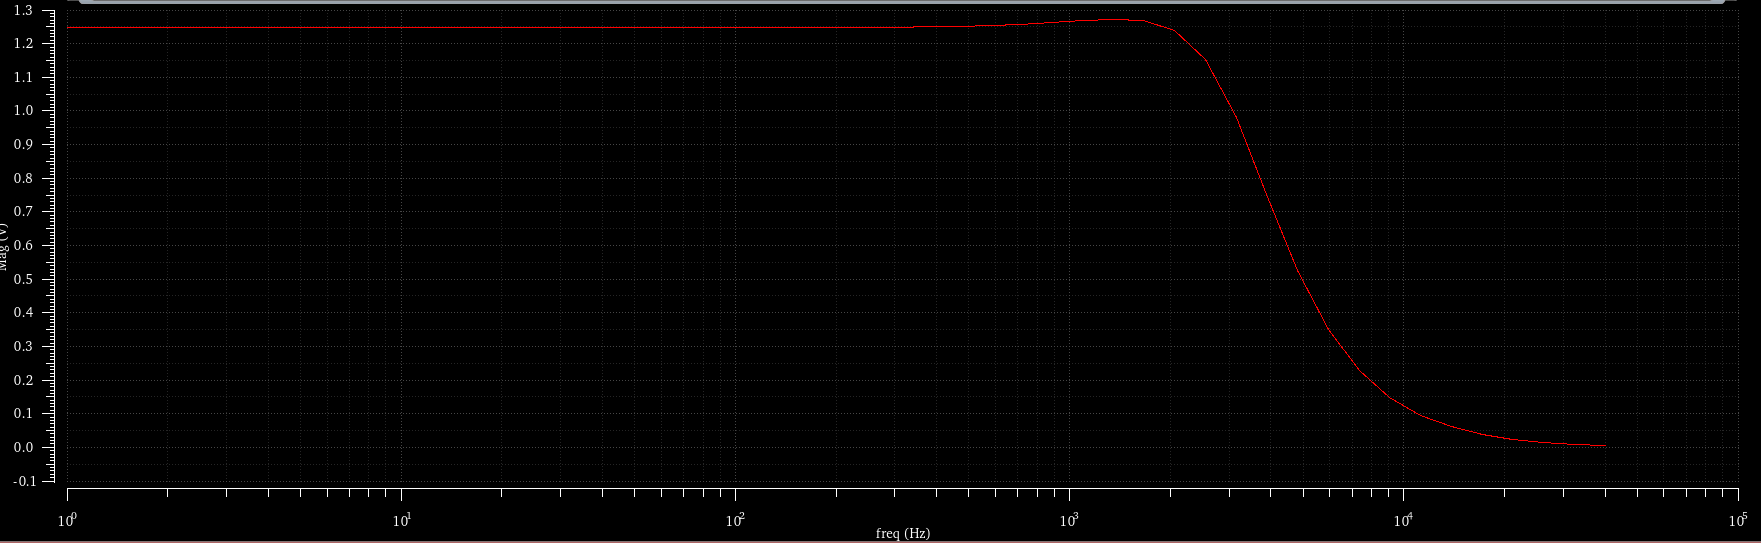
\includegraphics[width = 0.8\textwidth]{OriginalPlot}
    	\caption{初始仿真图像}
    \end{figure}\par
    分别考察$f_1 = 3kHz$与$f_2 = 35kHz$,不难验证满足需求。现在我们改变一些参量,观察其幅频特性的变化。
     \begin{figure}[H]
    	\centering
    	\subfigure[电压增益$A_v = 10$]{
    		\begin{minipage}[t]{0.48\linewidth}
    			\centering
    			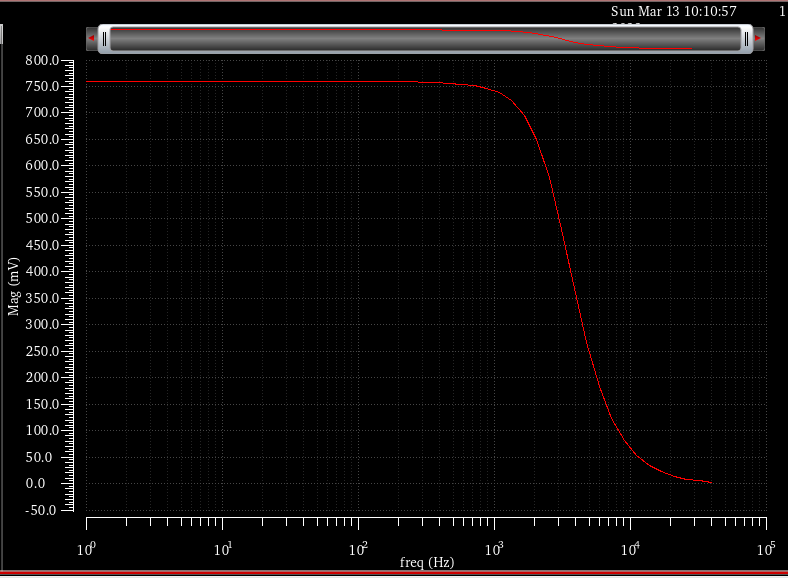
\includegraphics[width=6cm]{Av10}
    			% \caption{传输线LPF\ 50MHz-200MHz幅频特性}
    			%\caption{fig1}
    		\end{minipage}%
    	}
    	\subfigure[电压增益$A_v = 1000G$]{
    		\begin{minipage}[t]{0.48\linewidth}
    			\centering
    			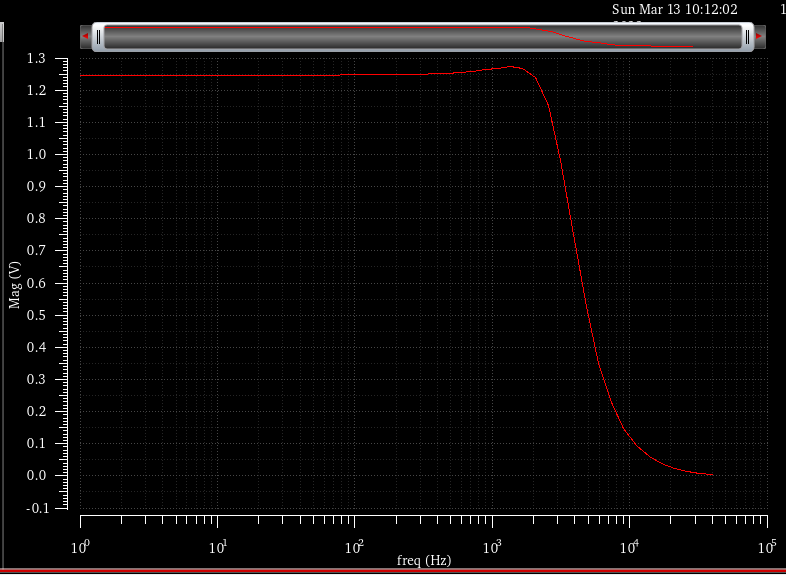
\includegraphics[width=6cm]{Av1000G}
    			% \caption{传输线LPF\ 50MHz-500MHz幅频特性}
    			%\caption{fig2}
    		\end{minipage}%
    	}%
    	%这个回车键很重要 \quad也可以 
    	
    	\centering
    	\caption{修改电压增益后的幅频特性}
    \end{figure}\par
     \begin{figure}[H]
    	\centering
    	\subfigure[单位增益频点$f_{unity\ gain} = 100Hz$]{
    		\begin{minipage}[t]{0.48\linewidth}
    			\centering
    			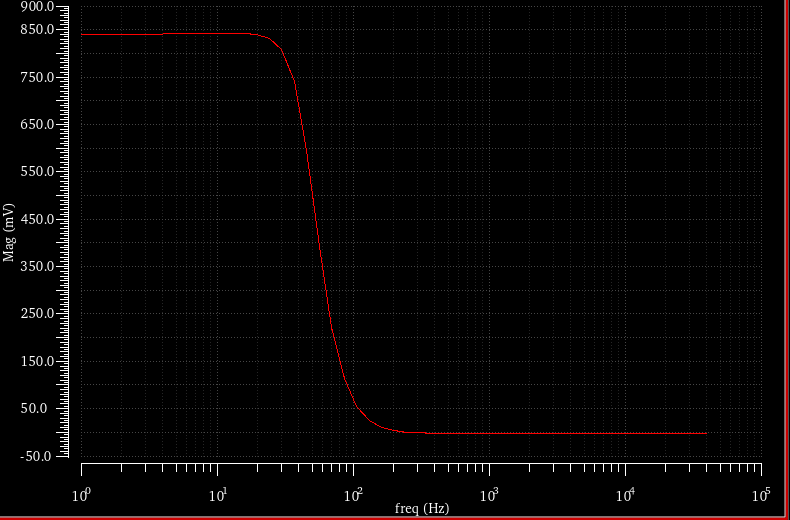
\includegraphics[width=6cm]{f100}
    			% \caption{传输线LPF\ 50MHz-200MHz幅频特性}
    			%\caption{fig1}
    		\end{minipage}%
    	}
    	\subfigure[单位增益频点$f_{unity \ gain} = 100GHz$]{
    		\begin{minipage}[t]{0.48\linewidth}
    			\centering
    			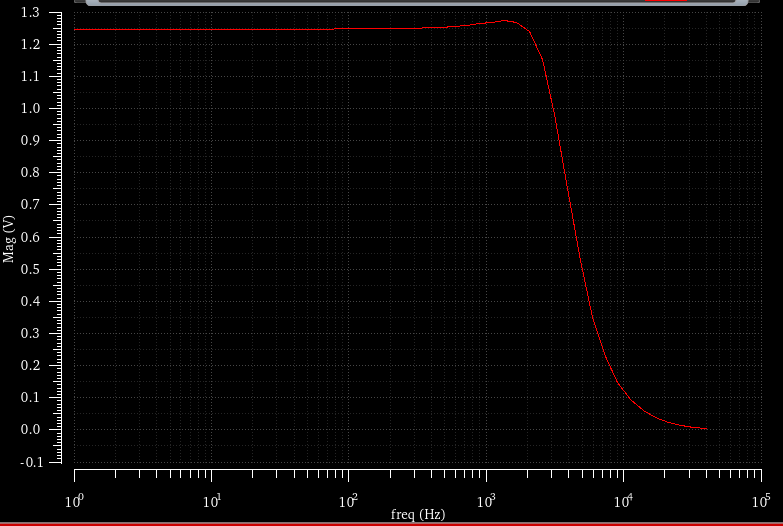
\includegraphics[width=6cm]{f100G}
    			% \caption{传输线LPF\ 50MHz-500MHz幅频特性}
    			%\caption{fig2}
    		\end{minipage}%
    	}%
    	%这个回车键很重要 \quad也可以 
    	
    	\centering
    	\caption{修改单位增益频点后的幅频特性}
    \end{figure}\par
     \begin{figure}[H]
    	\centering
    	\subfigure[输入电阻$r_i = 10 \Omega$]{
    		\begin{minipage}[t]{0.48\linewidth}
    			\centering
    			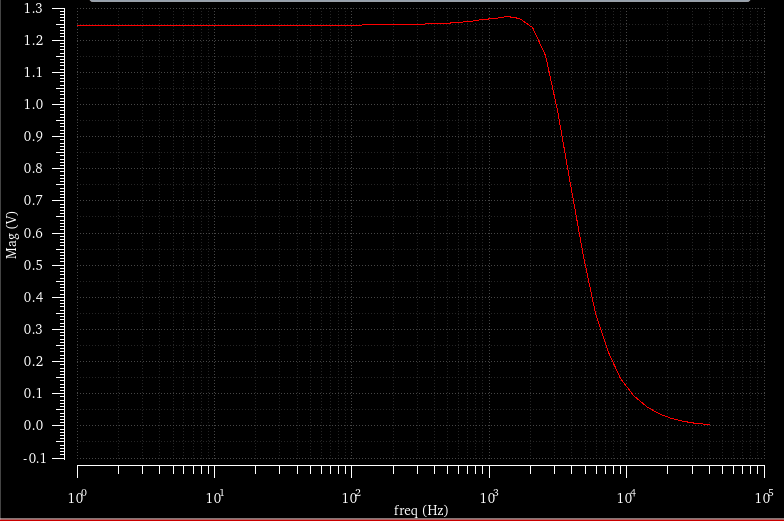
\includegraphics[width=6cm]{rin10}
    			% \caption{传输线LPF\ 50MHz-200MHz幅频特性}
    			%\caption{fig1}
    		\end{minipage}%
    	}
    	\subfigure[输入电阻$r_i = 100G\Omega$]{
    		\begin{minipage}[t]{0.48\linewidth}
    			\centering
    			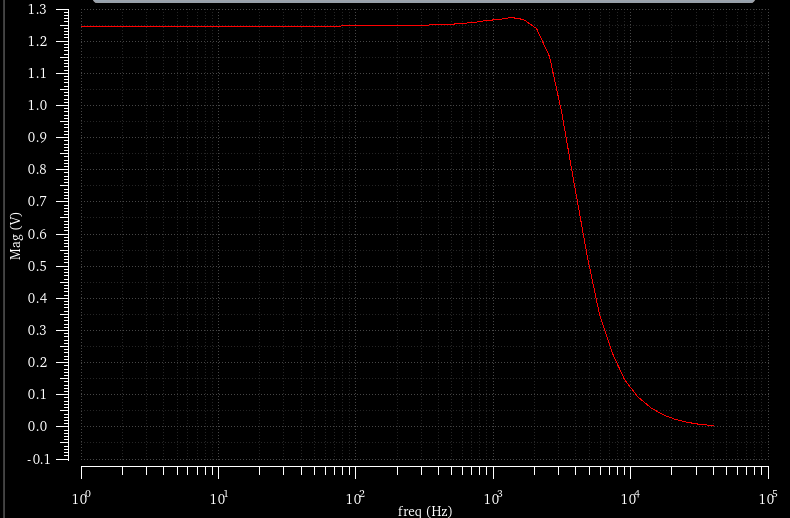
\includegraphics[width=6cm]{rin100G}
    			% \caption{传输线LPF\ 50MHz-500MHz幅频特性}
    			%\caption{fig2}
    		\end{minipage}%
    	}%
    	%这个回车键很重要 \quad也可以 
    	
    	\centering
    	\caption{修改输入电阻后的幅频特性}
    \end{figure}\par
    \begin{figure}[H]
    	\centering
    	\subfigure[输出电阻$r_o = 1k \Omega$]{
    		\begin{minipage}[t]{0.48\linewidth}
    			\centering
    			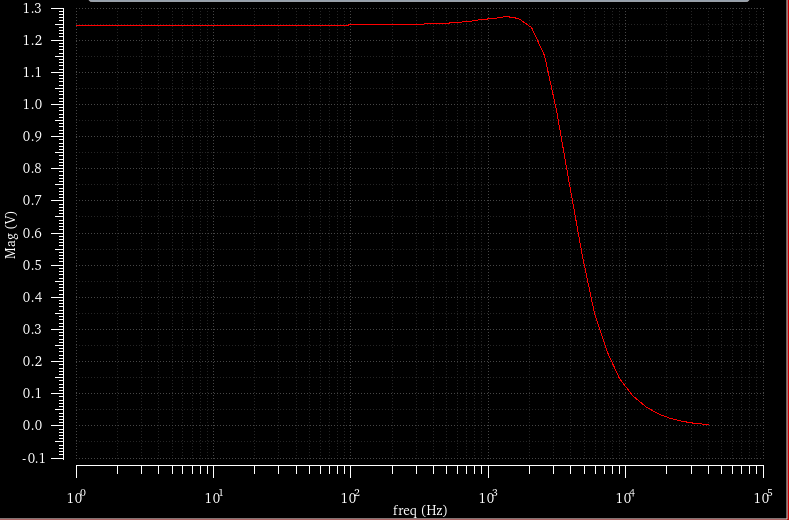
\includegraphics[width=6cm]{rout1k}
    			% \caption{传输线LPF\ 50MHz-200MHz幅频特性}
    			%\caption{fig1}
    		\end{minipage}%
    	}
    	\subfigure[输入电阻$r_o = 1G\Omega$]{
    		\begin{minipage}[t]{0.48\linewidth}
    			\centering
    			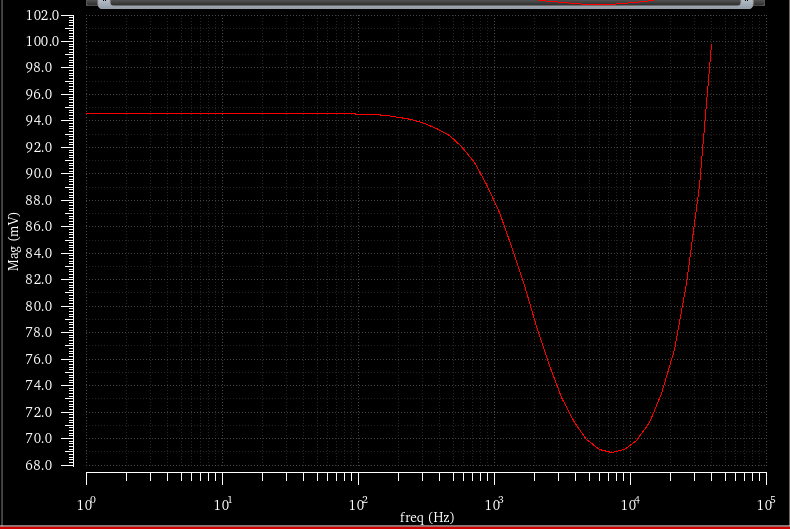
\includegraphics[width=6cm]{rout1G}
    			% \caption{传输线LPF\ 50MHz-500MHz幅频特性}
    			%\caption{fig2}
    		\end{minipage}%
    	}%
    	%这个回车键很重要 \quad也可以 
    	
    	\centering
    	\caption{修改输出电阻后的幅频特性}
    \end{figure}\par
    \section{CS、CD、CG、cascode放大器电压增益分析}
     \begin{figure}[H]
    	\centering
    	\subfigure[CS组态放大器]{
    		\begin{minipage}[t]{0.48\linewidth}
    			\centering
    			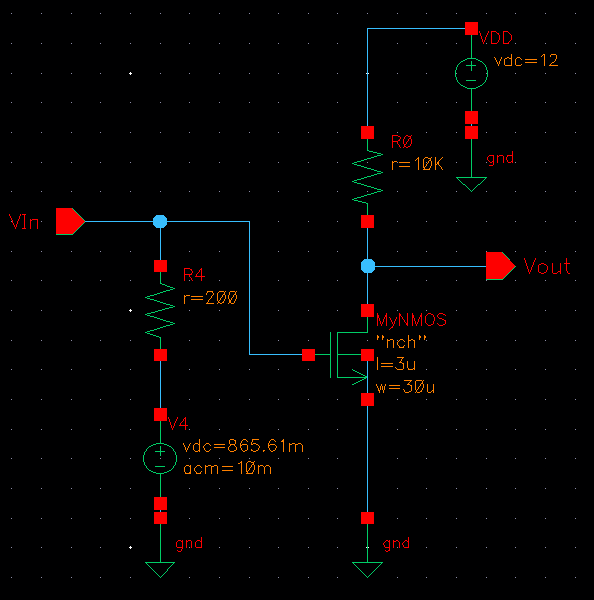
\includegraphics[width=6cm]{CS}
    			% \caption{传输线LPF\ 50MHz-200MHz幅频特性}
    			%\caption{fig1}
    		\end{minipage}%
    	}%
    	\subfigure[CG组态放大器]{
    		\begin{minipage}[t]{0.48\linewidth}
    			\centering
    			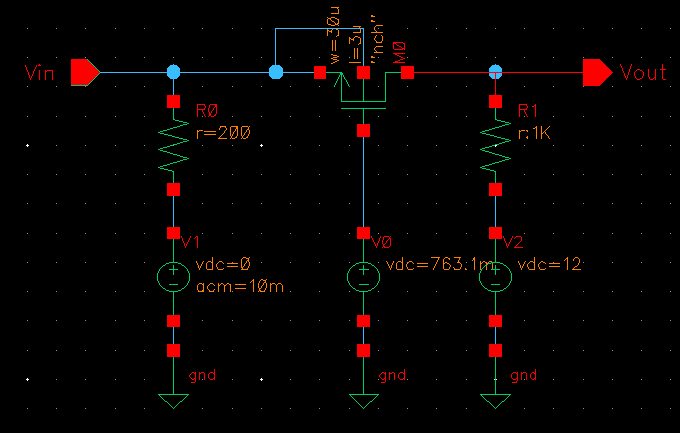
\includegraphics[width=6cm]{CG}
    			% \caption{传输线LPF\ 50MHz-500MHz幅频特性}
    			%\caption{fig2}
    		\end{minipage}%
    	}%
    	%这个回车键很重要 \quad也可以 
    	\par
    	\subfigure[CD组态放大器]{
    		\begin{minipage}[t]{0.48\linewidth}
    			\centering
    			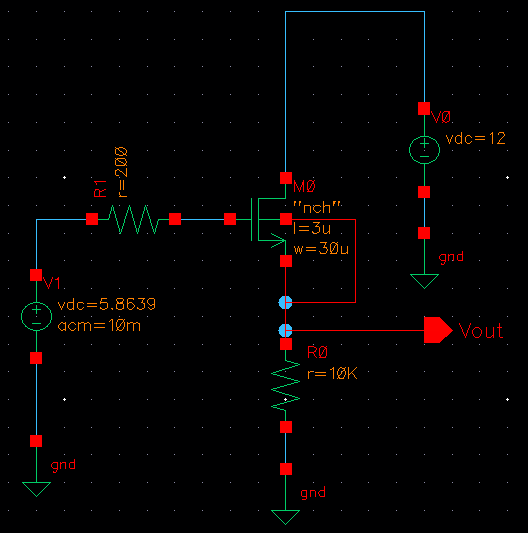
\includegraphics[width=6cm]{CD}
    			% \caption{传输线HPF\ 50MHz-200MHz幅频特性}
    			%\caption{fig2}
    		\end{minipage}
    	}%
    	\subfigure[cascode放大器]{
    		\begin{minipage}[t]{0.48\linewidth}
    			\centering
    			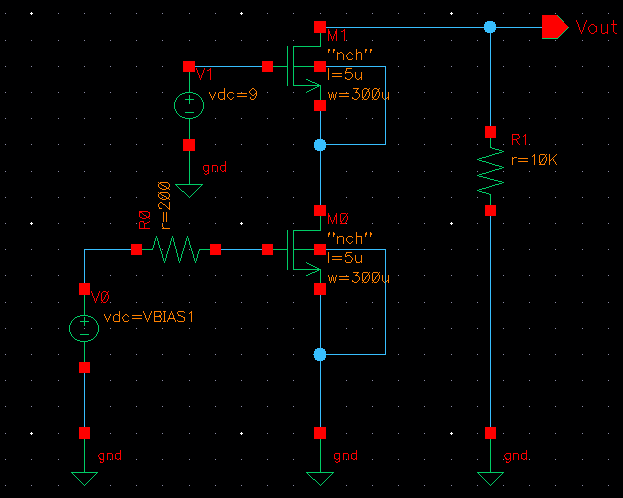
\includegraphics[width=6cm]{cascode}
    			% \caption{传输线HPF\ 50MHz-1GHz幅频特性}
    			%\caption{fig2}
    		\end{minipage}
    	}%
    	
    	\centering
    	\caption{四种基本放大器}
    \end{figure}\par
    \begin{figure}[H]
    	\centering
    	\subfigure[CS组态放大器直流工作点]{
    		\begin{minipage}[t]{0.48\linewidth}
    			\centering
    			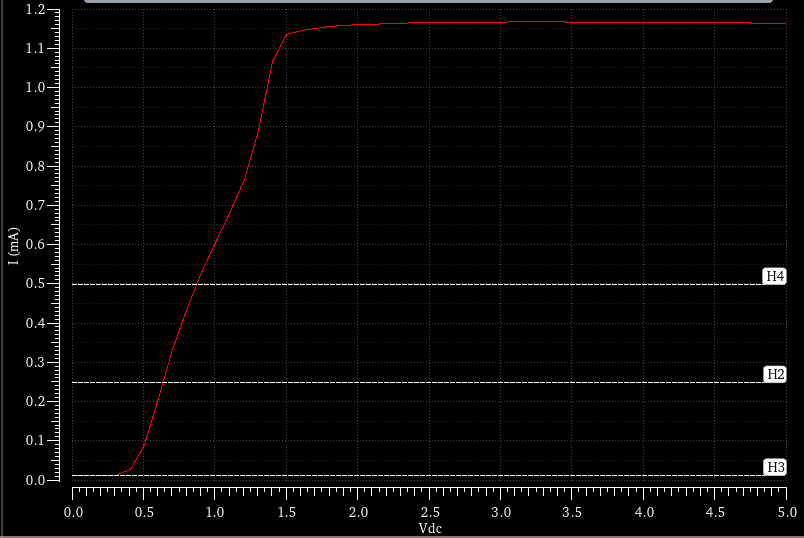
\includegraphics[width=6cm]{CS-DC}
    			% \caption{传输线LPF\ 50MHz-200MHz幅频特性}
    			%\caption{fig1}
    		\end{minipage}%
    	}%
    	\subfigure[CG组态放大器直流工作点]{
    		\begin{minipage}[t]{0.48\linewidth}
    			\centering
    			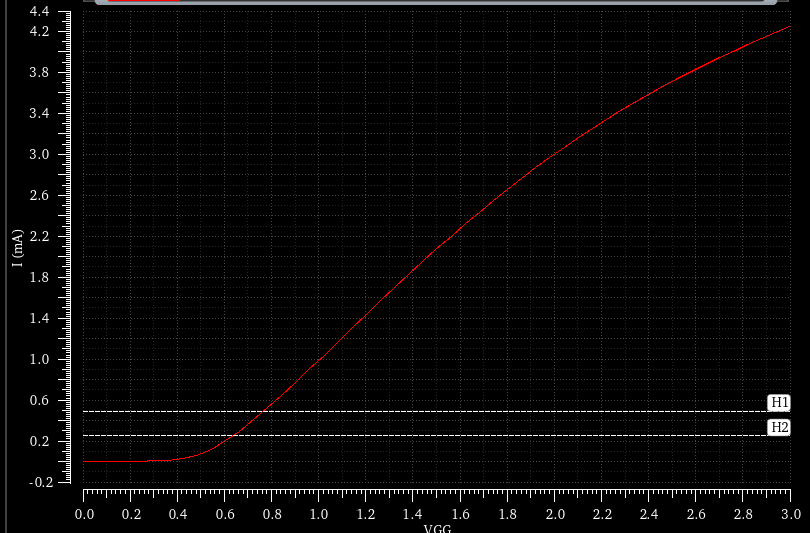
\includegraphics[width=6cm]{CG-DC}
    			% \caption{传输线LPF\ 50MHz-500MHz幅频特性}
    			%\caption{fig2}
    		\end{minipage}%
    	}%
    	%这个回车键很重要 \quad也可以 
    	\par
    	\subfigure[CD组态放大器直流工作点]{
    		\begin{minipage}[t]{0.48\linewidth}
    			\centering
    			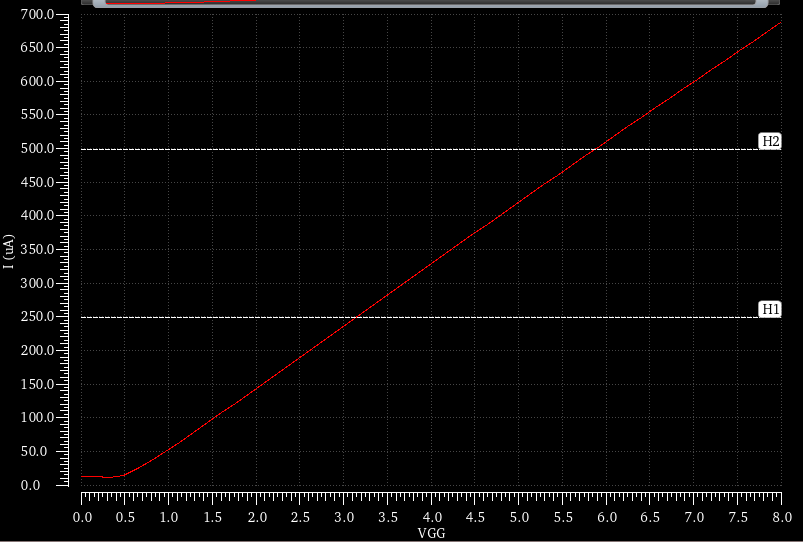
\includegraphics[width=6cm]{CD-DC}
    			% \caption{传输线HPF\ 50MHz-200MHz幅频特性}
    			%\caption{fig2}
    		\end{minipage}
    	}%
    	\subfigure[cascode放大器直流工作点]{
    		\begin{minipage}[t]{0.48\linewidth}
    			\centering
    			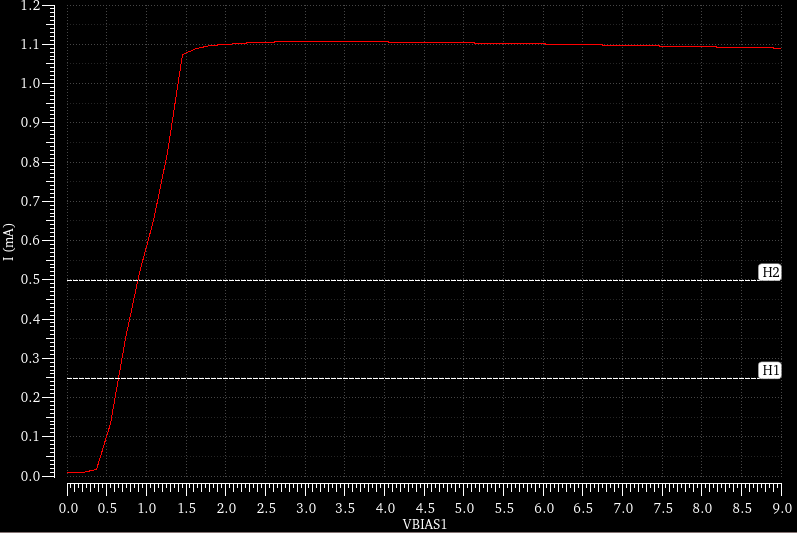
\includegraphics[width=6cm]{cascode-DC}
    			% \caption{传输线HPF\ 50MHz-1GHz幅频特性}
    			%\caption{fig2}
    		\end{minipage}
    	}%
    	
    	\centering
    	\caption{四种基本放大器直流工作点分析}
    \end{figure}\par
    \begin{figure}[H]
    	\centering
    	\subfigure[CS组态放大器交流增益]{
    		\begin{minipage}[t]{0.48\linewidth}
    			\centering
    			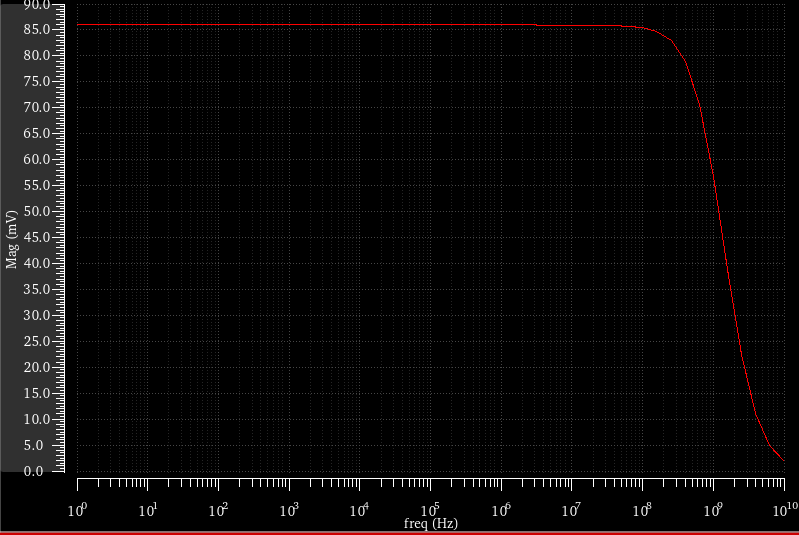
\includegraphics[width=6cm]{CS-AC}
    			% \caption{传输线LPF\ 50MHz-200MHz幅频特性}
    			%\caption{fig1}
    		\end{minipage}%
    	}%
    	\subfigure[CG组态放大器交流增益]{
    		\begin{minipage}[t]{0.48\linewidth}
    			\centering
    			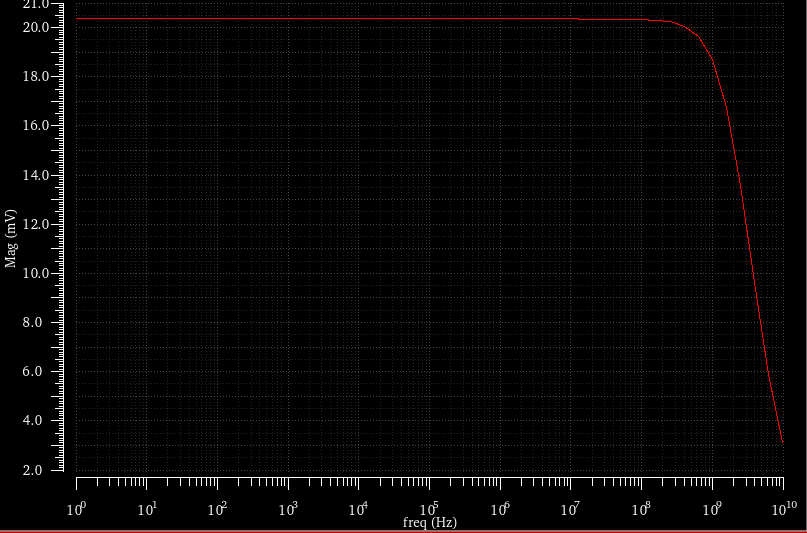
\includegraphics[width=6cm]{CG-AC}
    			% \caption{传输线LPF\ 50MHz-500MHz幅频特性}
    			%\caption{fig2}
    		\end{minipage}%
    	}%
    	%这个回车键很重要 \quad也可以 
    	\par
    	\subfigure[CD组态放大器交流增益]{
    		\begin{minipage}[t]{0.48\linewidth}
    			\centering
    			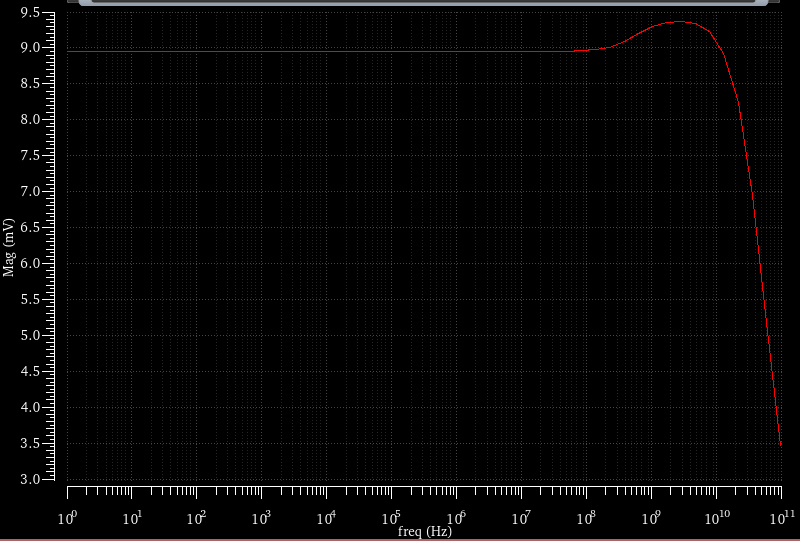
\includegraphics[width=6cm]{CD-AC}
    			% \caption{传输线HPF\ 50MHz-200MHz幅频特性}
    			%\caption{fig2}
    		\end{minipage}
    	}%
    	\subfigure[cascode放大器交流增益]{
    		\begin{minipage}[t]{0.48\linewidth}
    			\centering
    			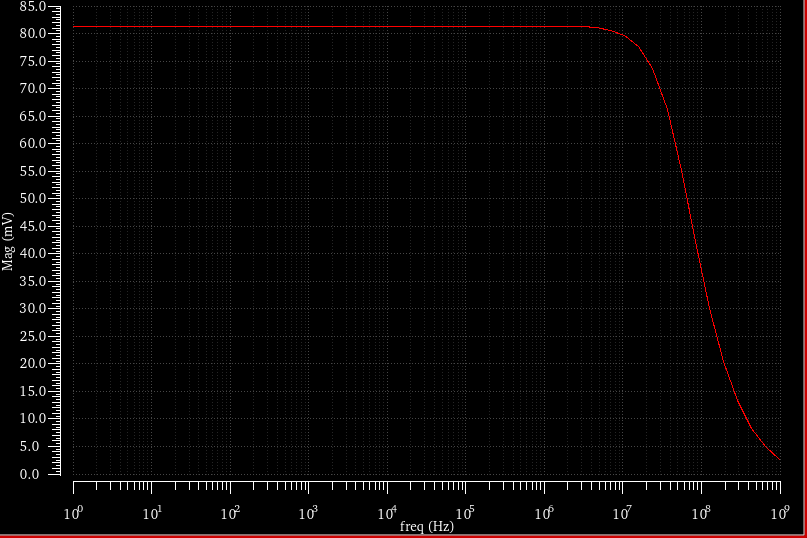
\includegraphics[width=6cm]{cascode-AC}
    			% \caption{传输线HPF\ 50MHz-1GHz幅频特性}
    			%\caption{fig2}
    		\end{minipage}
    	}%
    	
    	\centering
    	\caption{四种基本放大器交流增益分析}
    \end{figure}\par
\end{document}